%!TEX program = xelatex
\documentclass[a4paper,UTF8]{ctexart}
\usepackage[unicode=true,colorlinks,urlcolor=blue,linkcolor=blue,bookmarksnumbered=true]{hyperref}
\usepackage{latexsym,amssymb,amsmath,amsbsy,amsopn,amstext,amsthm,amsxtra,color,multicol,bm,calc,ifpdf}
\usepackage{graphicx}
\usepackage{diagbox}   % 绘制表格斜线
\usepackage{enumerate}
\usepackage{epstopdf}
\usepackage{fancyhdr}
\usepackage{subfigure}
\usepackage{listings}
\usepackage{multirow}
\usepackage{makeidx}
\usepackage{xcolor} 
\usepackage{fontspec}                            % 建立索引宏包
\graphicspath{{figures/}}  % 设置图片搜索路径
\theoremstyle{plain} \newtheorem{theorem}{定理}[section]
\theoremstyle{plain} \newtheorem{definition}{定义}[section]
\theoremstyle{plain} \newtheorem{lemma}{引理}[section]
\theoremstyle{plain} \newtheorem{proposition}{命题}[section]
\theoremstyle{plain} \newtheorem{example}{例}[section]
\theoremstyle{plain} \newtheorem{remark}{注}[section]
\theoremstyle{plain} \newtheorem{corollary}{推论}[section]
\newfontfamily\courier{Courier New}
\lstset{linewidth=1.1\textwidth,
        numbers=left, %设置行号位置 
        basicstyle=\small\courier,
        numberstyle=\tiny\courier, %设置行号大小  
        keywordstyle=\color{blue}\courier, %设置关键字颜色  
        %identifierstyle=\bf,
        commentstyle=\it\color[cmyk]{1,0,1,0}\courier, %设置注释颜色 
        stringstyle=\it\color[RGB]{128,0,0}\courier,
        %framexleftmargin=10mm,
        frame=single, %设置边框格式  
        backgroundcolor=\color[RGB]{245,245,244},
        %escapeinside=``, %逃逸字符(1左面的键),用于显示中文  
        breaklines, %自动折行  
        extendedchars=false, %解决代码跨页时,章节标题,页眉等汉字不显示的问题  
        xleftmargin=2em,xrightmargin=2em, aboveskip=1em, %设置边距  
        tabsize=4, %设置tab空格数  
        showspaces=false %不显示空格  
        basicstyle=\small\courier
       }  
\newenvironment{mysolution}{{\color{blue} 解}: }{{\color{magenta}\qed}}
\newcommand\diff{\,{\mathrm d}} %定义微分d
\newcommand{\p}[3]{\frac{\partial^{#1}#2}{\partial{#3}^{#1}}}  %定义求偏导算子
\newcommand{\ucite}[1]{\textsuperscript{\cite{#1}}}  %参考文献引用:上标用\ucite{ },文中用\cite{ }

\begin{document}
\title{

\includegraphics[width=0.65\textwidth]{onepiece.pdf}\\
\vspace{2em}
\textbf{K-Means 聚类学习笔记}}
\author{\emph{李向阳} \quad {\color{blue} d1142845997@gmail.com} }
\date{}


\maketitle
\thispagestyle{empty}

\newpage


\tableofcontents

\newpage

\section{引入}
前面我们主要讲的是分类问题(有监督学习), 也涉及到了预测(线性回归)和聚类(EM 算法). 这一次来介绍 K-Means 聚类方法, 由于比较简单且之前接触过, 因此本次的目的是稍微介绍 K-Means 聚类并对聚类算法(无监督学习)做一个系统的小总结.

其实我们在数据分析方法的课上已经学过了部分聚类分析, 包括快速聚类法与谱系聚类法, 这些都是根据样本聚类, 在课程里我们我简单讨论了按变量(特征)聚类. 事实上, 下面要讲的 K-Means 聚类就是我们学过的快速聚类法.


\section{基本框架}
在聚类(Cluster)分析中, 我们的样本是$\bm{x} = (x_1, x_2, \cdots, x_{n})^{T}$, 其中假设样本有$n$特征, 由于聚类是无监督学习, 自然也就没有类标签了. 设总共有$m$个样本, 为$\bm{x}_1, \bm{x}_2, \cdots, \bm{x}_m$,其中
\begin{equation*}
\bm{x}_i = (x_{i1}, x_{i2}, \cdots, x_{in})^{T}, i = 1,2, \cdots, m
\end{equation*}

假设每个特征的取值都是连续的数值型数据, 则每个样本都可看成是$n$维空间中的一个点, $m$个样本组成$n$维空间的$m$个点. 我们希望把相似的样本归为一类, 而衡量各样本之间的靠近程度, 自然可以用各个样本点之间的距离. 定义距离的方式有很多, 比如欧氏距离等等, 具体可以回顾数据分析方法.


\section{K-Means 聚类}
我们已经提到, 其实 K-Means 聚类就是快速聚类. 该方法首先将样本粗糙的分类, 然后再根据样本间的距离按一定规则逐步调整直到收敛. 快速聚类法适合样本数目较大的数据集做聚类分析, 不过需要事先指定分类的数目$K$. 我们知道, 快速聚类主要分为两步, 第一步是选择初始聚点, 第二步是不断进行迭代. 至于初始聚点(种子)的选择, 其实是影响很大的, 这个留到下面会用图像实例说明. 至于迭代过程, 在数据分析方法课上已经讲过了, 我们这里从机器学习的角度来推导出这个过程.

我们假设一共有$m$个样本, 最后要聚成$K$个 cluster. K-Means 方法的基本假设是: 对于每一个 cluster , 我们可以选出一个中心点(center), 使得该 cluster 中的所有的点到该中心点的距离小于到其他 cluster 的中心的距离. 虽然实际情况中得到的数据并不能保证总是满足这样的约束, 但这通常已经是我们所能达到的最好的结果, 而那些误差通常是固有存在的或者是由问题本身的不可分性造成的. 设第$k$个 cluster 中心点的坐标为$\bm{\mu}_{k}$, 则 K-Means 的代价函数为
\begin{equation*}
J = \sum_{i = 1}^{m} \sum_{k = 1}^{K} r_{ik} ||\bm{x}_{i} - \bm{\mu}_{k}||^2
\end{equation*}

其中$r_{ik}$在样本点$\bm{x}_{i}$被归类到第$k$个 cluster 时取值为$1$, 否则为$0$. 

因此 K-Means 的模型参数便是所有的$r_{ik}$和$\bm{\mu}_{k}$, 我们的目的便是通过极小化代价函数$J$来求得参数估计. 然而, 直接寻找$r_{ik}$和$\bm{\mu}_{k}$来极小化$J$并不容易, 这里我们可以采用类似 EM 算法中迭代求解的思想: 先固定$\bm{\mu}_{k}$, 选择最优的$r_{ik}$; 下一步则固定$r_{ik}$, 求出最优的$\bm{\mu}_{k}$. 如此不断反复迭代直到收敛即可.

先看第一步, 即固定$\bm{\mu}_{k}$, 选择最优的$r_{ik}$, 此时$J$是$r_{ik}$的线性函数, 而且每个样本$\bm{x}_{i}$其实是独立的, 因此我们可以极小化每一项来最小化$J$. 显然, 当$||\bm{x}_{i} - \bm{\mu}_{k}||^2$最小时我们让相应的$r_{ik}$为$1$, 其他情况让$r_{ik}$为$0$, 这样就最小化$J$了. 也就是说我们只要将样本点归类到离它最近的那个中心就能保证$J$最小, 即
$$
r_{ik} = 
\begin{cases}
1, & \textrm{当} k = \arg \min_{j} ||\bm{x}_{i} - \bm{\mu}_j||^2 \\ 
0, & \textrm{其他情况}
\end{cases}
$$


再看第二步, 即固定$r_{ik}$, 求出最优的$\bm{\mu}_{k}$. 直接将$J$对$\bm{\mu}_{k}$求梯度并令梯度为零即可.
\begin{equation*}
\nabla_{\bm{\mu}_k} J = \sum_{i=1}^{m} -2 r_{ik} (\bm{x}_{i} - \bm{\mu}_{k}) = 0
\end{equation*}

由此解得
\begin{equation*}
\bm{\mu}_{k} = \frac{\sum_{i=1}^m r_{ik} \bm{x}_i}{\sum_{i=1}^{m} r_{ik}}
\end{equation*}

也就是说$\bm{\mu}_{k}$的值是第$k$个 cluster 中所有数据点的平均值. 这刚好就是快速聚类的步骤.

由于每一次迭代都是取到$J$的最小值, 因此$J$只会不断减小或者不变, 达到一定程度之后就可以停止了.

下面我们举一个具体的例子, 来说明 K-Means 的具体过程. 原始数据如图\ref{rowdata}所示.
\begin{figure}[!htb]
	\centering
	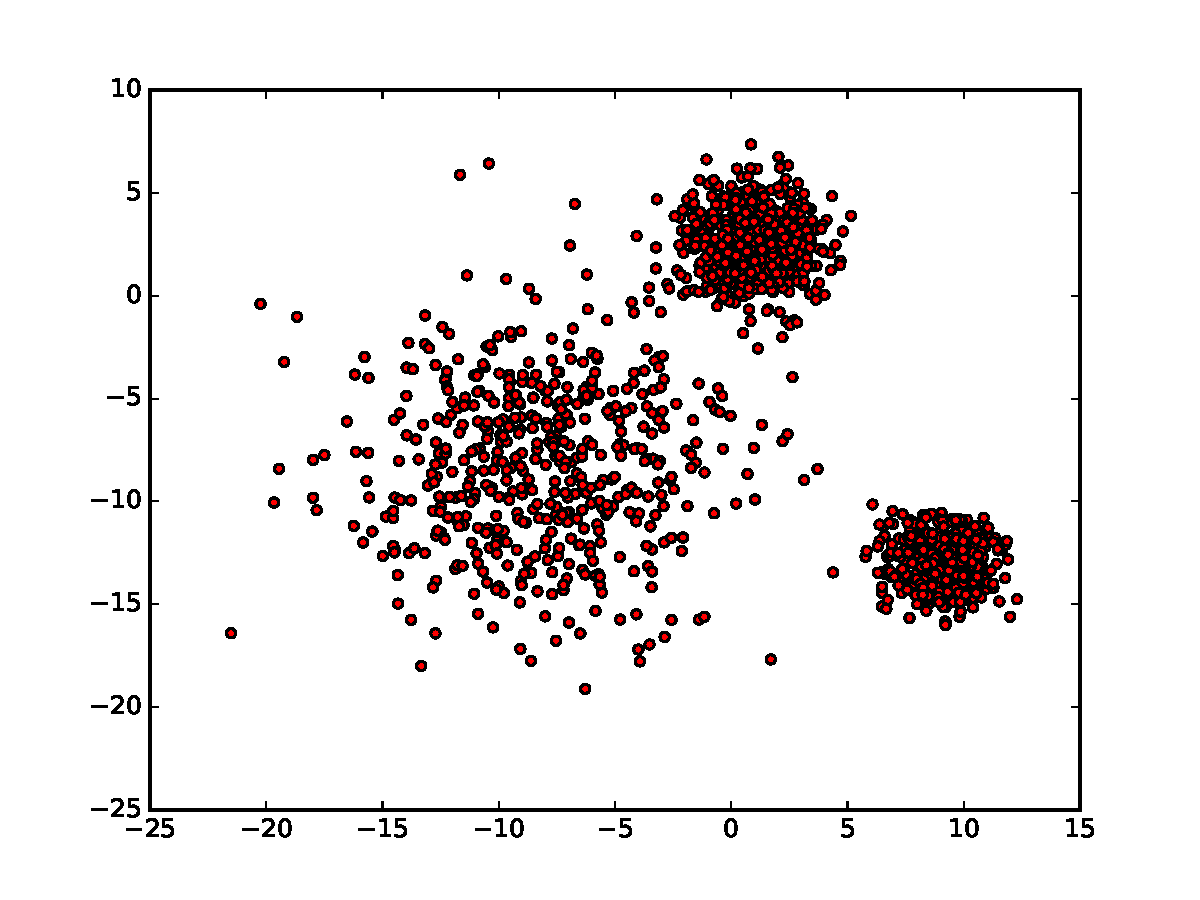
\includegraphics[width = 0.75 \textwidth]{rowdata.pdf}
	\caption{原始数据散点图}
	\label{rowdata}
\end{figure}

这里其实是用$3$个高斯分布生成的, 也就是其实是聚成$3$个类. 我们先随机选择初始聚点, 如图\ref{iter00}所示.
\begin{figure}[!htb]
	\centering
	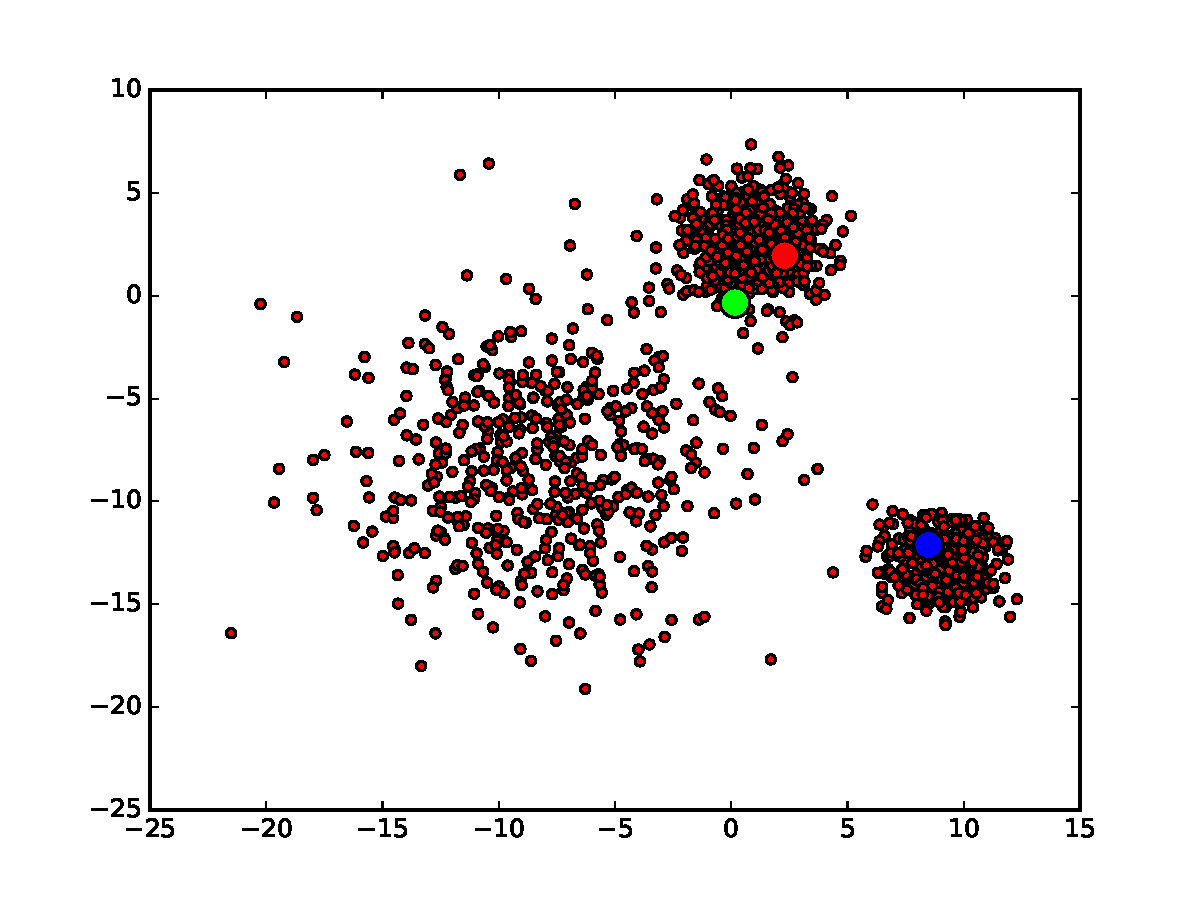
\includegraphics[width = 0.75 \textwidth]{iter_00.pdf}
	\caption{选择初始聚点}
	\label{iter00}
\end{figure}


则经过一次迭代, 可得图\ref{iter01}.
\begin{figure}[!htb]
	\centering
	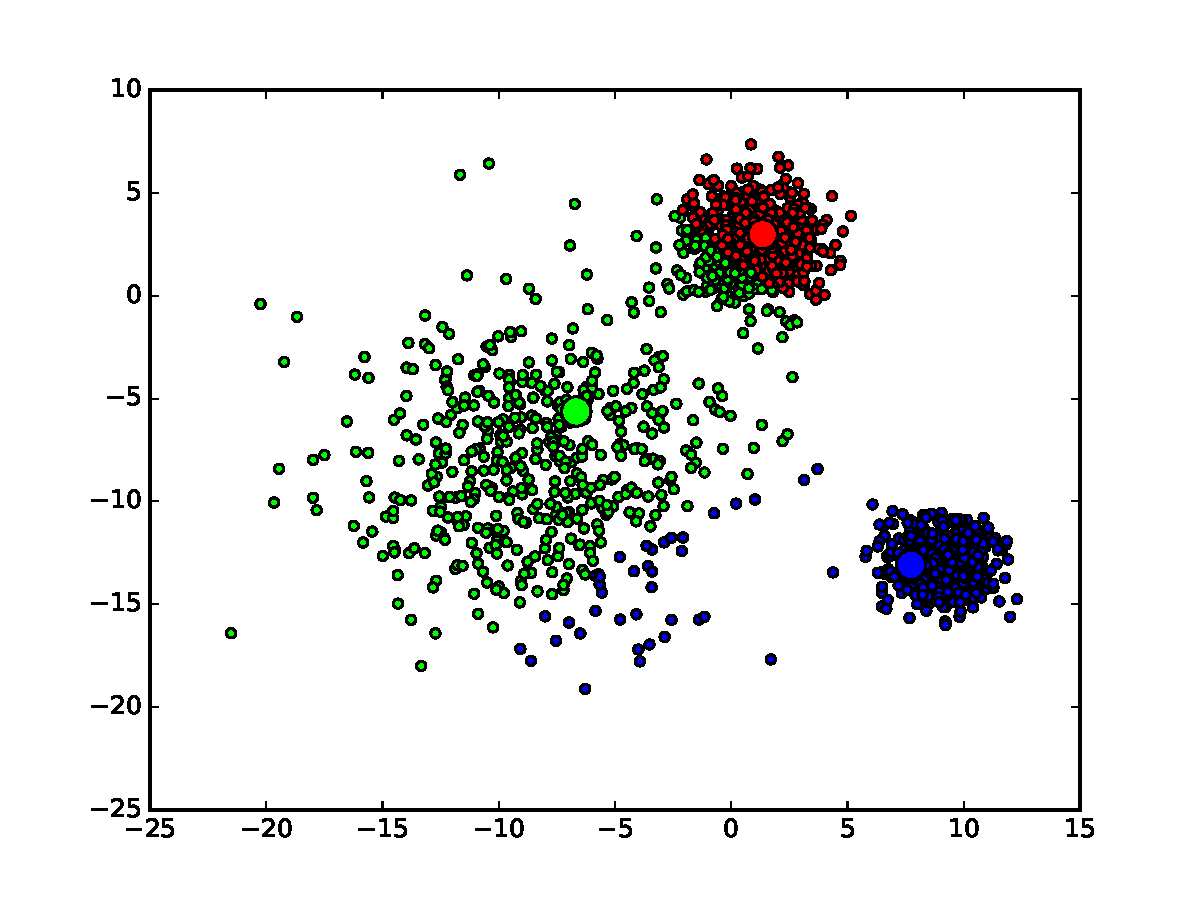
\includegraphics[width = 0.75 \textwidth]{iter_01.pdf}
	\caption{第一次迭代}
	\label{iter01}
\end{figure}

由于初始聚点选择的较好, 因此迭代几次便收敛了, 最终得到图\ref{iter04}.
\begin{figure}[!htb]
	\centering
	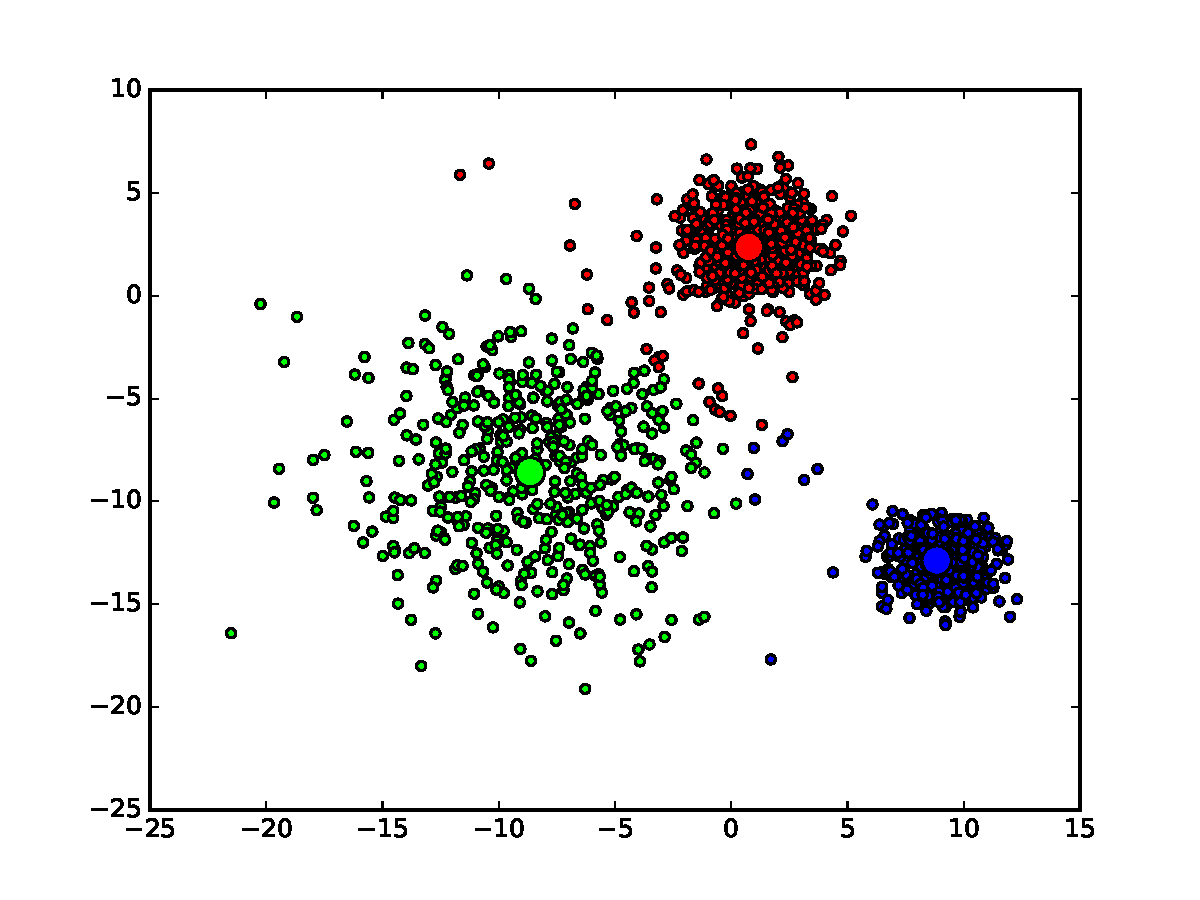
\includegraphics[width = 0.75 \textwidth]{iter_04.pdf}
	\caption{最终聚类图}
	\label{iter04}
\end{figure}

之前我们提到初始聚点的选择很关键, 比如对于本例子, 如果初始聚点的选择如图\ref{iter10}所示, 那么迭代计算可得最终的聚类图是图\ref{iter13}.
\begin{figure}[!htb]
	\centering
	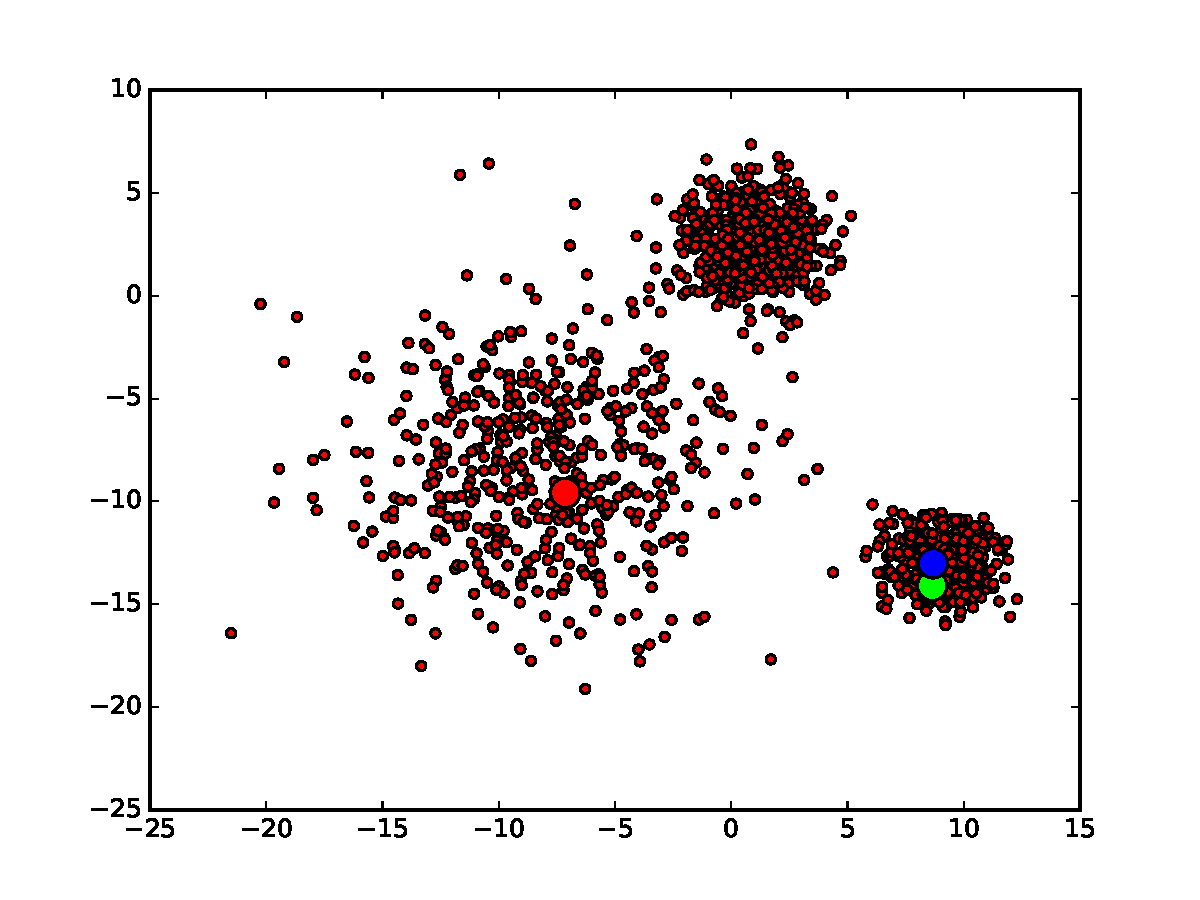
\includegraphics[width = 0.75 \textwidth]{iter_10.pdf}
	\caption{不好的初始聚点}
	\label{iter10}
\end{figure}

\begin{figure}[!htb]
	\centering
	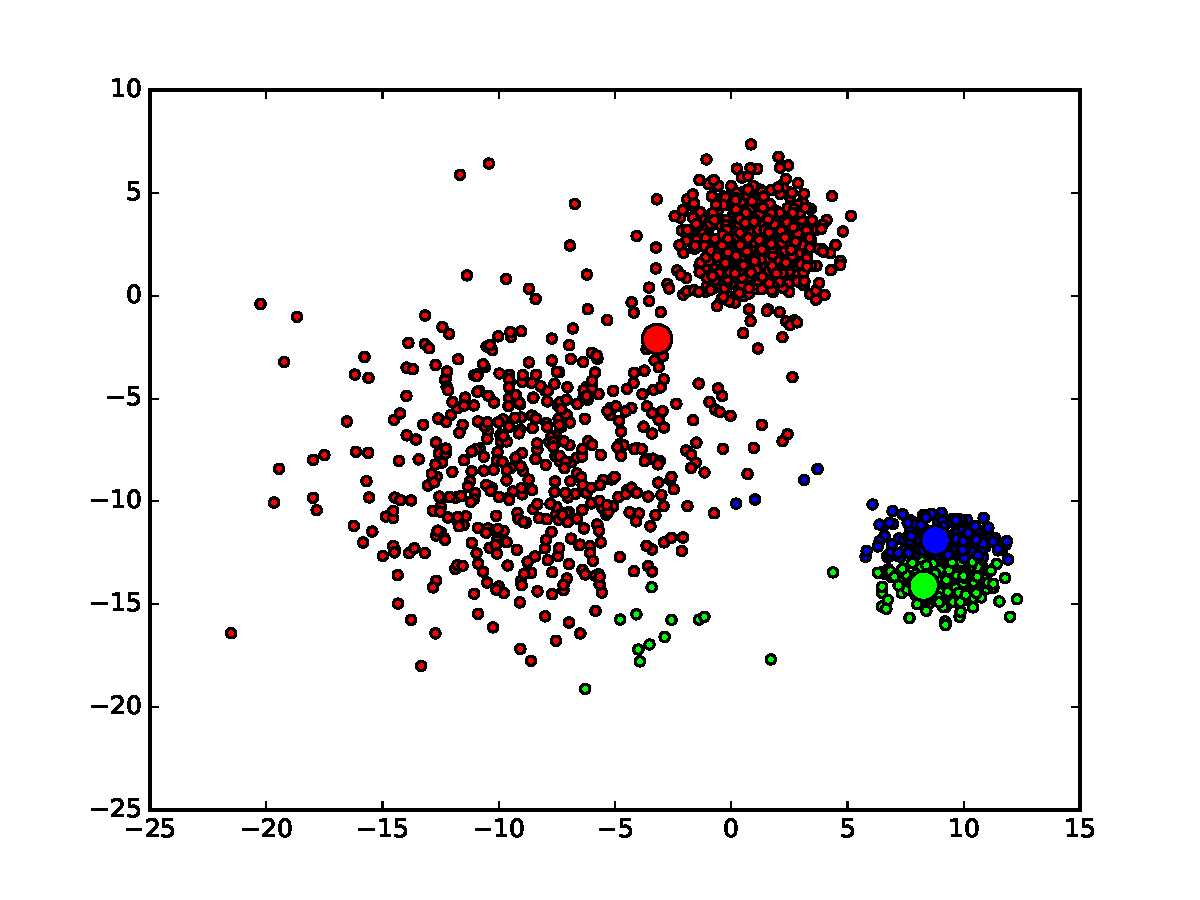
\includegraphics[width = 0.75 \textwidth]{iter_13.pdf}
	\caption{最终聚类图}
	\label{iter13}
\end{figure}

显然, 这并不是一个很好的结果. 而且讽刺的是, 这时也只迭代了$3$次就停止了. 我就不展示中间结果了. 基本的 K-Means 聚类就介绍到这里.


\section{关于聚类的补充}
\subsection{K-Means 聚类的推广}
上面我们用的距离是欧氏距离. 在数据分析方法的课上, 我们知道还可以用$L_{m}$距离进行快速聚类, 特别的, 当选为$L_{1}$距离时, 对应的中心为中位数向量. 我们知道, 中位数具有较强的稳健性. 而且用欧氏距离的话, 要求每个特征的取值是连续的, 但实际问题中总有些特征的取值是离散的或者取值不是数值型的, 这就不便于使用欧氏距离, 于是引入了 K-Medoids 聚类算法.

在 K-Medoids 中, 我们把原来的目标函数$J$中的欧氏距离改为一个任意的 dissimilarity measure 函数$\mathcal{V}$:
\begin{equation*}
J = \sum_{i=1}^{m} \sum_{k=1}^{K} r_{ik} \mathcal{V}(\bm{x}_{i}, \bm{\mu}_{k})
\end{equation*}

最常见的方式是构造一个距离矩阵$D$来代表$\mathcal{V}$, 其中元素$d_{ij}$表示样本$\bm{x}_i$与$\bm{x}_j$之间的差异程度(距离).

一般而言, K-Medoids 算法中的中心点是在已有的数据点里面选取的, 因此相对于 K-Means 来说, 不容易受到那些由于误差之类的原因产生的 outlier 的影响, 更加 robust 一些. 不过同 K-Means 一样, 初始聚点不好的时候效果也会很差.


\subsection{分级聚类(Hierarchical Clustering)}
分级聚类其实就是我们学过的谱系聚类法(也称系统聚类法). 谱系聚类法首先视各个样本自成一类, 然后把最相近(距离最小)的样品聚为小类, 再将已聚合
的小类按其相近性(用类间距离度量)再聚合, 随着相近性的减弱, 最后将一切子类都聚合成一个大类, 从而得到一个按相近性大小聚结起来的谱系图, 再进一
步根据实际情况确定合适的分类个数. 

谱系聚类的关键是依据样本间的距离定义类与类间的距离, 从而按照类间距离从小到大进行聚类. 我们当时在数据分析方法课上讲了最短距离、最长距离、类平均距离和重心距离等$4$种方法并得出了计算类间距离的递推公式. 至于如何实施, 可以回顾课本.


\subsection{混合高斯聚类}
在讲 EM 算法的时候, 我们提到可以利用混合高斯模型(GMM)进行聚类. 其实很简单, 有了样本数据, 假定它们是由 GMM 生成出来的, 那么我们只要根据数据推出 GMM 的概率分布来就可以了, 然后 GMM 的$K$个 Component 实际上就对应了$K$个 cluster 了. 具体估计参数的话, 可以使用 EM 算法.

相对于 K-Means 聚类, GMM 所得的结果不仅仅是数据点的 label, 而且包含了数据点标记为每个 label 的概率, 很多时候这实际上是非常有用的信息.


\subsection{关于 K-Means 与 $k-$NN}
其实二者的区别还是很明显的, 虽然名称中都含有$k$. 但是 $k-$ NN 是一个分类算法, 是有监督学习, 而 K-Means 聚类是一个聚类算法, 是无监督学习.








\section{总结}
\subsection{参考资料}
\begin{enumerate}[(1)]
\item 博客: \url{http://blog.pluskid.org/?page_id=78}, pluskid 写的聚类系列博客, 还是不错的, 里面还提到了一些比较现代的聚类算法.

\item PRML: 其实 pluskid 的聚类系列博客部分是参考的 PRML 的第九章, 这才是本源.

\item stackexchange: \url{http://stats.stackexchange.com/questions/111145/how-to-fit-mixture-model-for-clustering}, 用 R 自带的 kmeans 函数做了聚类分析, 并有画图展示.

\item 维基: \url{https://en.wikibooks.org/wiki/Data_Mining_Algorithms_In_R/Clustering/Expectation_Maximization_(EM)}, 用了 R 的 mclust 包做了混合高斯聚类. 当然, Python 的 sklearn 包聚类函数的能力也很强.

\end{enumerate}





\begin{thebibliography}{4}
  \bibitem{1} 李荣华.\emph{偏微分方程数值解法}.高等教育出版社(2010) 
  \bibitem{2} Zhilin Li,Zhonghua Qiao,Tao Tang.\emph{Numerical Solutions of Partial Differential Equations-An Introduction to Finite Difference and Finite Element Methods}.(2011)
  \bibitem{3} 孙志忠.\emph{偏微分方程数值解法}.科学出版社(2011)
  \bibitem{4} 陆金甫 关治.\emph{偏微分方程数值解法}.清华大学出版社(2004)
  
\end{thebibliography}

\newpage

\section*{附录}








\end{document}